\documentclass{article}
\usepackage{hyperref}
\usepackage{graphicx}
\usepackage{wrapfig}
\usepackage{lscape}
\usepackage{rotating}
\usepackage{epstopdf}

\title{The Riscy Processor}
\author{Karan Bavishi, Mark Mansi, Suhas Pai, Preyas Shah}

\begin{document}

\maketitle

\section{Introduction}

We implement the RV64I set of instructions in the RISCV ISA\cite{riscv-isa}
with a superscalar, out-of-order core. Our implementation is optimized for
correctness. Our second goal was performance.  Our third goal was
synthesize-ability. 
%All goals have been compromised for the sake of completion.

In Section~\ref{sec:overview}, we provide a brief overview of our design. In
Section~\ref{sec:modules}, we talk about the design of each individual module
in detail. Section~\ref{sec:perf-policies} describes some of the policies we
designed and implemented to boost the performance of our processor. In
Section~\ref{sec:design-dec}, we discuss some interesting design decisions we
took and the rationale behind it. In Section~\ref{sec:design-chal}, we talk
about a few challenges that we ran into, which forced us to rethink our design.
Finally, in Section~\ref{sec:performance}, we discuss the performance achieved
by our processor for certain benchmarks.

\section{Overview}
\label{sec:overview}

\begin{itemize}
    \item 4-wide pipeline
    \item Out-of-order execution; In-order commit
    \item Fetch
        \begin{itemize}
            \item 3 cycle latency for cache hit (2 cycle I-cache latency)
            \item Branch prediction (TODO): 2-level predictor, BTB, global
                history register.
            \item I-Cache: Blocking, 4 KB, 2-way associative, 1 read/write port.
            \item Prefetch Buffer: 4 entries, 32 bytes each
        \end{itemize}
    \item Decode and Rename
        \begin{itemize}
            \item 64-entry ROB
            \item 2 cycle latency
        \end{itemize}
    \item Issue and FUs
        \begin{itemize}
            \item 4 ALUs
            \item 4 issue queues, 16 entries each, 1 ALU per queue
            \item Load-balancing arbiter places new instructions in issue
                queues.
            \item ALUs also used to compute \texttt{ld}/\texttt{st} addresses.
        \end{itemize}
    \item Address Queue
        \begin{itemize}
            \item 32 entries
            \item Tracks load/store dependencies.
            \item Non-speculative memory disambiguation.
            \item Loads access cache out-of-order between stores.
            \item Stores access cache on commit.
            \item D-Cache (TODO)
        \end{itemize}
    \item Writeback
        \begin{itemize}
            \item Processor supports back-to-back execution of dependent
                instructions.
            \item Writeback structure (a.k.a ROB WB or more affectionately,
                \texttt{FooPP}) is designed to avoid the massive tangle of wires
                created by broadcast-based writeback among 4 ALUs and a LSQ.
        \end{itemize}
    \item Stall: we implement a distinct top-level module to handle stall
        coordination among all stages. The two stall producers in the pipeline
        are the issue queue arbiter and the ROB. A stall is generated when there
        is not enough room in the issue queues or the ROB. Each stage is a
        consumer of stalls produced by stages before it.
\end{itemize}

\begin{figure}[ht]
	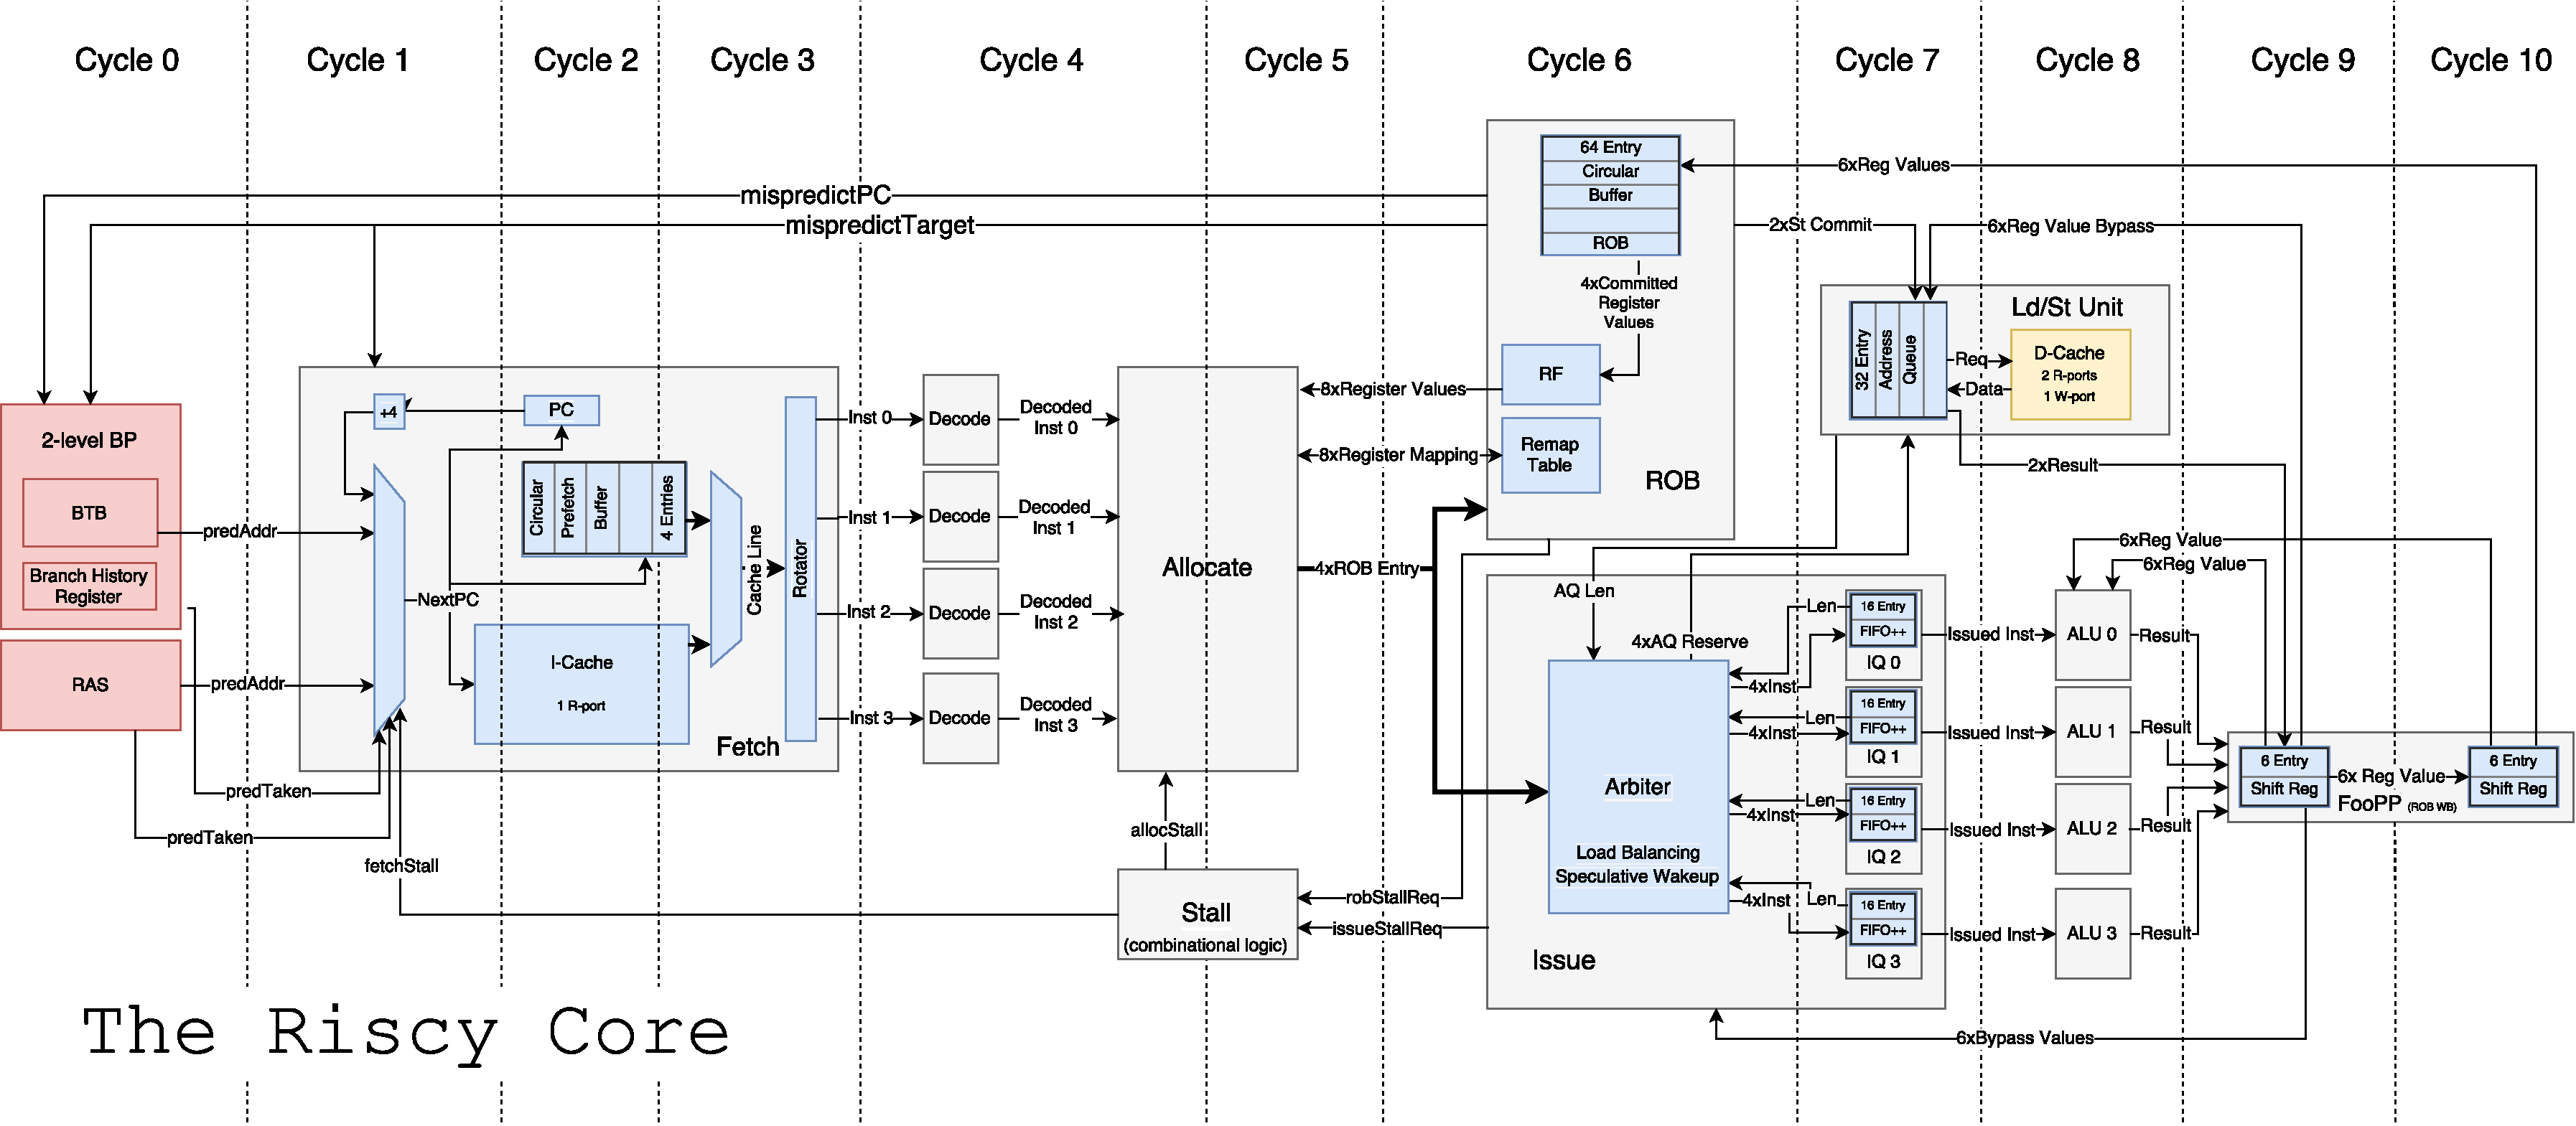
\includegraphics[page=1,width=1.25\textwidth]{riscy_diagram.pdf}
	\caption{Top-level diagram of our processor}
	\label{fig:top-level}
\end{figure}

A top-level diagram of our design is shown in Figure~\ref{fig:top-level}. A
bigger version of the diagram is also available for view\cite{riscy-diagram}.

\section{Modules}
\label{sec:modules}

Our processor has a pipeline depth of 8. The pipeline is divided into several
independently designed and implemented blocks (implemented as modules in
Chisel). This section presents an overview of the whole processor. Then, we
present the design of each block.

\subsection{Fetch}

Our fetch module encapsulates the logic of selecting the next PC, issuing
requests to the instruction memory hierarchy (including the I-cache), and presenting
instructions to the subsequent stage (decode).

We implement a pipelined, blocking, 2-way associative instruction cache with
2-cycle latency. And additional cycle of latency comes from computing the next
PC.

The instruction cache returns a hit if it finds the requested entry. If not, it
issues a refill request to memory for the missing address. Once the memory
responds, it refills its data and tag arrays with the response. The cache line
replacement policy is random replacement.  

We also added a prefetch buffer, containing 4 entries. It does cache block
prefetching ie. it stores the additional cache lines sent by memory as a part
of its response to a refill request. This is primarily done to get around the
single-port limitation of the I-cache. This prefetch buffer can be easily
changed to do next-line prefetching as a part of future work.

The output from the instruction cache is rotated and presented to the rest of
the pipeline.

\subsection{Decode and Allocate}

The next two cycles are consumed in decoding and renaming the instructions from
fetch.

Decode takes less than one cycle because it consists entirely of separating
wires. Thus, we combine decode with the first cycle of renaming.

Renaming proceeds in two phases. The first cycle decodes the instruction and
renames all destinations. The second cycle renames operands and produces and ROB
entry which can just be latched to the ROB next cycle.

\subsection{ROB}

The ROB is implemented as a 64-entry circular buffer. All committing logic is
implemented in the ROB module. 4 instructions can commit in a single cycle. In
the same cycle, 4 new ROB entries can also be added to the tail of the ROB.

We choose to use an ROB as opposed to a merged register file because we
prioritized performance and ease of implementation over energy.

\subsection{Issue and FUs}

In the same cycle, an ROB entry both latches in the ROB and goes to the issue
queue arbiter, which puts it in a queue. All instructions go through the arbiter
regardless of their type.

Our issue stage consists of an arbiter feeding 4 issue queues.
The arbiter does load balancing to attempt to keep any queue from becoming
filled while other ALUs are available.

Each issue queue is independent and feeds a single ALU. The issue queues can
each independently wake up a single instruction to be sent an ALU. Our
implementation is capable of speculatively waking up ALU operations when their
operands are known to be nearly ready. This allows our processor to execute
instruction with back-to-back dependencies. Our writeback mechanism helps with
this also...

\subsection{Writeback}

Each cycle, our processor may produce up to 6 values that need to be written
back (4 from ALUs and 2 from memory). To avoid creating $O(n^2)$ wires between
all of these value producers/consumers, we designed a single writeback
structure, which we call \texttt{FooPP}. All values are written back to the
\texttt{FooPP} in the cycle they produced. Any consumers of those values,
including the ROB and issue queues, take the values directly from the
\texttt{FooPP}.

To avoid adding a 1 cycle bubble between instructions with back-to-back
dependencies, the \texttt{FooPP} keeps 1 cycle of history, which the FUs can
then consume from easily.

The writeback structure also filters out any values coming from squashed
instructions. It does this by comparing the \emph{era} of the input values with
the \emph{current era} according to the ROB. This allows us to get rid of the
squashed instructions easily by letting them percolate through the pipeline.

\subsection{Address Queue}

When a load or store instruction reaches the arbiter, the arbiter asks the
address queue to reserve a spot for it. If the address queue is full, the
pipeline stalls. The arbiter then puts the load or store in a normal issue queue
to wait until an ALU can compute its address.

When the address is written to the Writeback structure, the address queue will
consume it.

Loads can access the D-cache as soon as their address is known and it is also
known that there is no preceding store to the same address.

Stores can access the D-cache as soon as the ROB signals the address queue that
they have committed.

To limit the number of ports need on the D-cache, we instead assume only two
ports. The ROB gives the guarantee that no more than 2 stores will commit in any
cycle.

\section{Performance Enhancement Policies}
\label{sec:perf-policies}

In this section, we talk about some of the design decisions we took which were
aimed at improving the performance of our processor. 

\begin{enumerate}
	\item Fetch - We added a prefetch buffer which stored cache blocks when
	a refill response was received from memory. This helped us get around
	the limitations of having a single-ported I-cache, which allowed us to
	only write one cache line when the refill response was received. Having
	a prefetch buffer allowed us to store multiple cache lines. 
	
	The prefetch buffer also helped improve performance by having enough
	instructions to keep the backend busy. Without the prefetch buffer, we
	were only able to serve instructions every 2 cycles before incurring
	another hit.
	
	\item Decode \& Allocate - Both Decode and Allocate stages were done in
	the same pipeline stage to avoid wasting a cycle
	
	\item Issue \& ROB - Renamed instructions are sent to both the ROB and
	Issue modules in parallel to save a pipeline stage. We also added
	support for speculative wakeup of instructions whose operands would be
	ready in the subsequent cycle via the ALU output. This allowed us to
	perform back-to-back execution for dependent instructions and boost
	performance.
	
	\item Execute - Apart from sending the ALU results to the ROB, the
	Writeback module was also responsible for storing the results for 2
	cycles for bypass. This bypass support allowed us to execute dependent
	instructions in back-to-back cycles.
	
	\item ROB mis-prediction eras - Incase of a mis-prediction, there are
	two ways to squash the speculated instructions. The first involves
	adding $O(n^2)$ valid bit wires everywhere, and resetting them when a
	mis-prediction occurs. The second way is to let the squashed
	instructions percolate through the pipeline. 
	
	The problem with the latter approach is that the ROB can not let new
	instructions pass through unless all the squashed instructions have
	percolated. This is because we can end up having new and squashed
	instructions with the same ROB tag. In order to get around this issue,
	we add misprediction eras. Whenever ROB realizes a misprediction, it
	increments the era counter. This era can help us distinguish between
	new instructions and to-be squashed instructions. 
\end{enumerate}

\section{Design Decisions}
\label{sec:design-dec}
In this section, we talk about the interesting design choices we made for our
processor.

\begin{enumerate}
	\item Pipelined Decode \& Rename - In our Decode and Allocate design,
	we decode and rename the destination in the first cycle.  Renaming of
	operands is done in the second cycle. This allows us to allocate new
	entries in the ROB in the second cycle, in parallel with the renaming
	of operands.
	
	\item Use Writeback to flush values from squashed instructions - As
	mentioned in Section~\ref{sec:perf-policies}, we decide to let the
	instructions to be squashed percolate through the pipeline.  An
	interesting question was to how to filter out the results from these
	squashed instructions and not make them be mistakenly used for bypass.
	We ultimately decided to add some filter logic to the Writeback module
	inputs. This made sure that the squashed values were invalidated and
	thus never available for bypass.
	
	\item Arbiter load-balancing and bypass - Our original idea was to have
	the arbiter build dependency graphs and put dependent instructions in
	the same queue. The rationale was that putting dependent instructions
	in the same queue would reduce the overhead of bypass across queues.
	However we soon realized that this plan would result in a multi-cycle
	arbiter design.
	
	We ultimately decided to have a simple arbiter which would issue
	instructions based on load balancing, i.e. instructions would be issued
	based on the emptiness of the queues. This allowed us to design a
	single-cycle arbiter. However, this brought back the original problem
	of complex bypass. For this, we designed the Writeback structure which
	would allow bypass of computed values to the 4 ALUs.
	
	\item LSQ: Use Issue queue wakeup logic for load/store instructions -
	Our original plan was to have 4 issue queues and 1 load-store queue,
	using 4 ALUs and 1 AGU. But we decided to re-use the existing ALUs for
	address computation for loads and stores.  This would allow us to
	re-use the complex instruction wakeup logic already present in the
	Issue Queues, and not re-implement from scratch.
	
	\item LSQ: Serialize loads and stores so that D-cache can have 1 read
	port and 2 write ports - TODO
	
	\item Unified Stall logic - We decided to come up with a unified stall
	module which would take stall requests as input from ROB and Arbiter
	modules and generate stall outputs to the consumers such as the Fetch
	and the I-cache modules. This unified logic simplified the interface
	between all these modules, and avoided complex wiring.
\end{enumerate}

\section{Design Challenges}
\label{sec:design-chal}
In this section, we talk about certain challenges that we encountered which
forced us to rethink our design. 

\begin{enumerate}
	\item Cancelling memory requests due to mispredictions - After adding
	misspeculation recovery support, we found that our processor had a
	5-cycle bubble before instructions were fetched from the new target. On
	investigating more, we realized that it was because the I-cache was
	busy requesting an address from memory that would no longer be needed.
	To get around this, we added support for cancellation of requests to
	memory incase of mispredictions.
	
	\item ROB deadlock issues - During testing, we saw the ROB running into
	weird deadlock issues. This forced us to rethink the question --
	\textit{what does it mean to stall for the ROB?} We realized that even
	if the ROB is stalled, it must continue to commit instructions to avoid
	deadlocks. 
	
	This helped solve our original problem where we saw our processor being
	deadlocked when the ROB stalled everything as soon as a stall request
	was issued by the LSQ via the Arbiter when it got full.
	
	\item Timing issues because of multiple fan-ins to Issue Queues - We
	had to carefully design the Issue Queue logic to ensure robustness to
	timing issues which were caused because of multiple fan-ins. If not
	done carefully, this could result in weird situations where the
	instructions would simply bounce off and not get stored in the Issue
	Queues.
		
	\item Zombie instructions eating up space - While adding support for
	misspeculation recovery through percolation, we realized that the
	squashed instructions (or zombie instructions) could end up staying
	much longer in the Issue Queue because of operands not being ready.
	Consider the case where a zombie load instruction is kept waiting for
	100 cycles waiting for the memory to respond to the request. This can
	happen because in our percolation policy, we execute the zombie
	instructions but decide to filter the results. 
	
	In order to get around this, we decided to add a special priority for
	zombie instructions in the instruction wakeup logic. This meant that
	zombie instructions lying in the Issue Queue were given the highest
	priority for wakeup, and thus would be percolated as soon as possible.
\end{enumerate}

\section{Performance}
\label{sec:performance}

\subsection{Methodology}
We ran a series of workloads to show the upper and lower bounds of IPC that our
processor could achieve. We ran the workloads in two main settings to test the
impact of lack of a data-cache and data-prefetching:
\begin{itemize}
\itemsep 0em
	\item 7 cycle memory latency
	\item 4 cycle memory latency (smallest possible latency supported by
	our design)
\end{itemize}

Additionally, we also ran the same workloads with instruction prefetching
turned on. In Section~\ref{sub:results}, we talk about the results achieved
with the two above-mentioned settings, and along with instruction-prefetching
wherever correctness of the benchmarks was verified.

\subsection{Benchmarks}
We ran multiple workloads which were aimed at highlighting the lower and upper
bounds of the IPC that could be achieved by our processor. In the following
table, we list the benchmarks that were used:

\begin{center}
    \begin{tabular}{ | p{1.8cm} | p{1.9cm} | p{1.75cm} | p{5cm} |}
    \hline
    Benchmark & ILP & Instructions & Description \\ \hline
    Counters (optimal) & High ILP & 8K insts & 32 counters incremented
    independently. \\ \hline
    Fibonacci & Max ILP 1.5 & 150 insts & Compute the first 64 Fibonacci
    numbers. \\ \hline
    Daxpy & High ILP (50 \% memory insts) & 3K insts & Element-wise addition of
    arrays. \\ \hline
    Stall (worst case) & Low ILP & 160 insts & Back-to-back dependent
    instructions force in-order execution \\
    \hline
    \end{tabular}
\end{center}

We describe the benchmarks and the reasons for choosing them in more detail below:
\begin{enumerate}
	\item \textit{Counters} - In this benchmark, we increment 32 counters
	independently. The reason for choosing this benchmark is to have as
	many independent instructions as possible and thus find out the upper
	limit of ILP that can be achieved by our design.

	\item \textit{Fibonacci} - The Fibonacci benchmark is aimed at testing
	our design with a purely compute-based workload. Due to the
	dependencies in the Fibonacci recurrence relation, the maximum ILP that
	can be achieved is 1.5.

	\item \textit{Daxpy} - We use a loop-unrolled version of the DAXPY
	benchmark. Since the original version involves multiply instructions
	which are not supported in our design, we multiply by 1 which is
	basically a no-op. This benchmark has a high ILP workload with a high
	memory-to-compute ratio of instructions, aimed at stressing the LSQ
	part of our design.

	\item \textit{Stall} - In this benchmark, we execute 160 back-to-back
	dependent instructions. The maximum ILP that can be achieved is 1. The
	rationale behind choosing this to verify that our design can execute
	dependent instructions in back-to-back cycles with no bubbles.
\end{enumerate}

\subsection{Results}
\label{sub:results}

In the following table, we describe the ILPs achieved for all the benchmarks in
the 2 chosen memory latency settings, with instruction prefetching enabled and
disabled. We omit results for settings where we were unable to verify
correctness.

\begin{center}
    \begin{tabular}{|l|c|c|c|c|}
    \hline
    Setting & Counters & Fibonacci & Daxpy & Stall \\ \hline
    7 cycle, I-prefetch disabled & 0.80 & 0.74 & 0.80 & 0.74 \\ \hline
    7-cycle, I-prefetch enabled & 2.22 & 1.30 & - & 0.91 \\ \hline
    4 cycle, I-prefetch disabled & 1.14 & 1.04 & 0.88 & 0.92 \\ \hline
    4 cycle, I-prefetch enabled & 2.66 & - & - & - \\
    \hline
    \end{tabular}
\end{center}

The following interesting observations can be made:
\begin{enumerate}
	\item \textit{Instruction prefetching makes a huge difference} - As can
	be seen from the ILP numbers achieved by our best-case Counters
	benchmark, it is hard to achieve a high ILP unless you have enough
	instructions to keep the backend busy. With instruction prefetching
	disabled, our processor incurs the memory latency penalty every 2
	cycles. 
	
	Interestingly, even with prefetching enabled, our design is only able
	to reach an ILP of 2.66. The reason for this is that our prefetching
	design is fairly naive -- it is not a next-line prefetcher. The
	prefetch unit does not fetch instructions well in advance and only
	stores additional cache lines when a penalty is incurred. If we
	increase the size of the prefetch buffer from 4 to 8, our projections
	show that we can achieve an ILP of about 3.2. 
	
	Having a more intelligent prefetcher and increasing the size of the
	prefetch buffer should help boost the ILP close to the maximum
	theoretical limit of 4. 
	
	\item \textit{Important to have a big instruction window} - Similar to
	our previous observation, it is extremely important to have a big
	instruction window to exploit the techniques implemented in an
	out-of-order design. Without enough instructions in the frontend, it is
	difficult to find enough parallelism and the processor remains hampered
	by dependencies and memory latencies.
		 
	\item \textit{Memory latency can significantly degrade the ILP} - As
	can be seen from the ILP numbers achieved by the Daxpy benchmark, it is
	hard to achieve a high ILP unless the memory latency can be hidden
	effectively.
	
	The Daxpy benchmark has an inherently high-ILP workload, but since our
	design lacks a data-cache, it is unable to go beyond executing more
	than one instruction per cycle.
	
	\item \textit{Close to optimal performance in Fibonacci} - We achieve
	an ILP of 1.30 for the 7-cycle, prefetching enabled setting, which is
	quite close to the theoretical limit of 1.5. We can actually reach an
	even higher figure of 1.42 for the 4-cycle, prefetching enabled
	setting, but we decided not to show it here because we couldn't get the
	correct result from the benchmark.
	
	\item \textit{Optimal performance in Stall} - Our Stall benchmark
	results are very close to the optimal ILP of 1.0. This highlights our
	processor's ability to execute dependent instructions in bac-to-back
	cycles with no bubbles.

\end{enumerate}


\begin{thebibliography}{9}

\bibitem{riscv-isa}
  RISCV ISA -  \url{https://riscv.org/specifications/}.
  
\bibitem{riscy-diagram}
  RISCY Core diagram - \url{https://github.com/mark-i-m/riscy/raw/master/riscy/doc/riscy_diagram.pdf}
  

\end{thebibliography}

\end{document}
